\documentclass[12pt,english]{article}
\usepackage{geometry}
\geometry{verbose,letterpaper,tmargin=2.4cm,bmargin=2.4cm,lmargin=2.4cm,rmargin=2.4cm}
\usepackage[T1]{fontenc}
\usepackage{lmodern}
\usepackage{amssymb,amsmath}
\usepackage{ifxetex,ifluatex}
\usepackage{natbib}
\bibliographystyle{plainnat}
\usepackage{graphicx}
\usepackage{caption}
\usepackage{subcaption}
\usepackage{brush_style}
\usepackage{setspace}
\usepackage{lineno}
\linenumbers
\title{Persistence of marine populations under climate and fishing}
\author{Emma Fuller$^1$, Eleanor Brush$^2$, Malin Pinsky$^{1,3}$}
\date{\small (1): Department of Ecology and Evolutionary Biology, Princeton University, Princeton, New Jersey 08544 USA \\
(2): Program in Quantitative and Computational Biology, Princeton University, Princeton, New Jersey 08544 USA \\
(3): Department of Ecology, Evolution and Natural Resources, Rutgers University, New Brunswick, New Jersey 08901 USA}

\begin{document}
\maketitle
\pagebreak
\begin{spacing}{1.9}
\begin{flushleft}

\section{Abstract}

When the climate changes, so does the location of habitats suitable for an organism's survival and reproduction. This change does not occur in isolation but rather appears on a background of other disturbances, making the study of interactions between stressors important. In order to understand how two disturbances, range shift and harvesting, interact and affect population persistence, we analyzed an integrodifference model that explicitly included the mechanisms of dispersal and reproduction. We found how the critical rates of harvesting and climate velocity depend on the growth rate and dispersal kernel of the population.  We measured the interaction between the stressors and found that the disturbances interact nearly additively, with low positive synergy only at the greatest harvest rates and climate velocity that almost drive the population extinct. We also introduced two conservation techniques into simulations of the population model --- threshold harvest rules and marine protected areas (MPAs) --- and found that under some circumstances these approaches could be effective management tools as they mitigate the interaction between the two stressors.  
\hspace{10cm}

\noindent {\bf Keywords:} Climate change, fishing, integrodifference model, synergy, multiple disturbances

\section{Introduction}

Many stressors can disturb an ecosystem, and ecologists have quantified the consequences of a great deal of these of perturbations \citep{Wilcoveetal1998, Crainetal2008, DarlingCote2008}. Less work, however, has been done to measure the effects of multiple stressors and the interactions between them.  If disturbances interact synergistically, a perturbation that has little effect when it occurs individually may amplify the disturbance caused by a coincident perturbation \citep{Crainetal2008, DarlingCote2008,Nyeetal2013,Gurevitchetal2000}.   In the most extreme (and worrying) cases, synergistic interactions between multiple stressors will drive a population extinct even though it could persist in the face of any single stressor (e.g. \citet{Pelletieretal2006}).  If disturbances interact antagonistically, on the other hand, the effects of multiple stressors may be less than that predicted by the individual effects of the stressors.  Since disturbances rarely occur in isolation, measuring the effects of multiple disturbances gives a better understanding of the likely impacts to the system \citep{DoakMorris2010, Fordhametal2013, Foltetal1999}.


Climate change and fishing, two of the largest human impacts on the ocean \citep{Halpernetal2008}, provide an important case study of how disturbances interact in their effects on biological populations.  Marine fish are already moving in response to climate change \citep{Perryetal2005, HiddinkHoftstede2008, Rijnsdorpetal2009, Dulvyetal2008, Simpsonetal2011} and are projected to continue in the future \citep{Kelletal2005, Mackenzieetal2007}. These shifting species, and those likely to move in the future, are also subject to harvesting, among other disturbances including pollution, ocean acidification, habitat fragmentation, and invasive species \citep{Wilcoveetal1998, Salaetal2000, MEA2005, Pinskyetal2013, Barryetal1995, Nyeetal2009}. Previous empirical work has found synergistic interactions between overfishing and temperature-driven range shifts \citep{Lingetal2009} and microcosm experiments have identified synergistic interactions between warming temperatures, harvesting and connectivity \citep{Moraetal2007}. This empirical work underscores the importance of understanding how range shifts and harvesting interact. 

A common approach to predicting future population distributions has been to use bioclimatic-envelope models (also known as species distribution models -- SDMs). These statistical models typically correlate presence-absence data with biophysical characteristics such as mean or maximum temperatures, rainfall, or salinity, to predict how species ranges' will differ under climate change \citep{Elithetal2006, GuisanThuiller2005, GuisanZimmerman2000}. Despite these models' widespread adoption, many papers have criticized SDMs as oversimplified as they lack species interactions, dispersal and reproductive processes \citep{KearneyPorter2009, Zarnetskeetal2012, Robinsonetal2011}.  Recent work on range shifts has addressed some of these gaps by explicitly including dispersal and reproduction \citep{Berestyckietal2009, ZhouKot2011}. However these models only address one disturbance, climate-driven range shifts.

Work on the joint impacts of climate and fishing often considers climate fluctuations (large anomalies around the mean) rather than directional changes in climate \citep{WaltersParma1996, KingMcFarlane2006}. When studies consider the effects of climate-driven range shifts on fishing, the models are typically case-specific and detailed, integrating multiple drivers and disturbances \citep{Cheungetal2010, Lindegrenetal2010, Brownetal2010, Merinoetal2010, Merinoetal2010b, Plaganyietal2011, Ainsworthetal2011, Zhangetal2011, Barangeetal2011, Howardetal2013}. These predicted impacts are important for management and conservation planning \citep{Allisonetal2009}, however these models are so complex that it makes understanding the relative importance of particular drivers, disturbances, and interactions difficult (but see \citet{Nyeetal2013} for an approach using ecosystem-level models to discern relative importance of disturbances).

Here we extended a previously studied model of a fish population subject to climate-driven range shift by also considering harvesting pressure. The model explicitly included reproduction and dispersal, two mechanistic processes central to species' responses to climate and fishing. Previous work has highlighted the importance of these two processes and their vulnerability to climate change \citep{Fordhametal2013, Hastingsetal2005}.  We found the critical harvesting rate and climate velocity that drive the population extinct and how these critical rates depend on one another.   We also found that climate-driven range shifts and fishing interact nearly additively, with low positive synergy at more extreme levels of the stressors.  

We also examined the efficacy of two different types of management strategies: threshold harvesting rules and marine protected areas (MPAs). MPAs are frequently recommended for conservation of biodiversity and improved fisheries yield \citep{Gainesetal2010}, and we evaluate whether MPAs established for those purposes could improve species persistence when habitat shifts rapidly.  Previous work has suggested protected areas can be a key form of climate insurance and can provide stepping stones to help species keep up with a changing environment \citep{Thomasetal2012, Hannahetal2007}.  We found that threshold harvesting rules remove the interaction between harvesting rates and climate velocity and that MPAs can help a species persist with higher harvesting pressure and slightly increase the maximum climate velocity with which a species can keep up.

\section{Methods}

We studied the dynamics of a fish population constrained to a single, one-dimensional habitat patch by their inability to reproduce outside of that area as introduced by \cite{ZhouKot2011}. This viable habitat patch (here after `patch') shifts at a fixed velocity and harvest occurs at each point in space along the entire one-dimensional world.  We first determined the climate velocity and harvesting rate that would drive the population extinct (hereafter the critical harvesting rate and climate velocity), and then measured synergy by calculating the drop in biomass caused by each stressor both individually and together. We finally add marine protected areas (MPAs) and threshold harvesting rules in numerical simulations of the model to determine how these management strategies affect population persistence.

\subsection{The Model }

In the model of \cite{ZhouKot2011}, the adults from the current year produce offspring according to a recruitment function and these offspring disperse across the one-dimensional world according to a dispersal kernel to become the next generation's adults.  We extend this model by additionally subjecting the adults to harvesting before they produce offspring so that only a proportion of the fish survive to reproduce. We incorporate these processes-- recruitment, harvesting, and dispersal-- into an integrodifference model to describe how the population changes over time. If $n_t(x)$ 
is the density of fish at position $x$ at time $t$, then the density of fish at the next generation is given by

\begin{equation*}
n_{t+1}(x)=\int^{\frac{L}{2}+ct}_{-\frac{L}{2}+ct}k(x-y)f((1-h)n_t(y))dy \label{integrodifference},
\end{equation*}

\noindent where $h$ is the proportion of adults harvested, $f(n)$ is the recruitment function giving the number of 
offspring produced by a population of size $n$ (accounting for density dependence), $k(x-y)$ is the dispersal kernel giving the probability of a  larva traveling from position $y$ to position $x$, $L$ is the length of the patch, and $c$ is the rate at which it  shifts across space.  We provide a list of variables and functions in Table \ref{variables}.  We use a Beverton-Holt recruitment function,

\[f(n_t)=\frac{R_0n_t}{1+\left(\frac{R_0-1}{K}\right)n_t}\]  

\noindent but regardless of the exact functional form of the recruitment function, the critical parameter in determining population persistence is how quickly recruitment increases when the population size is near (but above) $0$, which is equivalent to the intrinsic growth rate $R_0=f'(0)$.  Analyzing this kind of model becomes easier if the dispersal kernel is separable into its dependence on the source of larvae and its dependence on the destination of the larvae, i.e.~if there are functions $a_i, b_i$ such that $k(x- y) = \sum^\infty_{i=1} a_i(x)b_i(y)$.  In our analyses, as in \cite{Latore:1998fk}, we used the separable Gaussian kernel given by

\[k(x-y)=\frac{1}{2\sqrt{D\pi}}e^{\frac{-(x-y)^2}{4D}}.\]

\noindent To derive analytical expressions, we approximated the kernel, as described in the Appendix. %section number necessary?
Analytical results for a separable sinusoidal kernel are also described in the Appendix.  %awkward
We used simulations to analyze a Laplace dispersal kernel that is not amenable to this method, as described below.  % Why did we choose a Laplace dispersal kernel for simulations? 

At equilibrium, a traveling wave will describe the population, where the density of fish at a given point in space will change but the density of fish at a location relative to the shifting patch will not. We sought to describe  the distribution of the population over the viable patch as it shifts through the world in order to study the size of the population at equilibrium and whether or not the population could persist. The traveling wave $n^*$ must satisfy

\begin{equation}
n^*(\bar{x})=\int^{\frac{L}{2}}_{-\frac{L}{2}}k(\bar{x}+c-\bar{y})f((1-h))n^*(\bar{y}))d
\bar{y}, \label{traveling_pulse}
\end{equation}

\noindent where $\bar{x}\in\left[-\frac{L}{2}, \frac{L}{2}\right]$ describes the position within the patch \citep{ZhouKot2011}.

\subsection{Persistence }
One possible equilibrium traveling wave that solves Equation (\ref{traveling_pulse}) is the `trivial' traveling pulse, $n^*(\bar{x}) = 0$ for all $x \in \left[-\frac{L}{2}, \frac{L}{2}\right]$, i.e.~a patch with no fish in it.  If a population persists, it must be able to avoid extinction and grow even when small. We can think of a small population as a perturbation to the trivial traveling pulse. If the trivial pulse is stable, the system will return to the trivial pulse even after the introduction of a small population. If the trivial pulse is unstable, a small population may increase and form a persistent population. Population persistence is therefore equivalent to the trivial traveling pulse being an unstable equilibrium.   

If we harvest the population at low enough levels and the climate velocity is slow enough, the population will be able to persist.  There exists threshold values of the harvesting rate $h$ and a climate velocity $c$ such that if we increase parameters beyond these values, we drive the population extinct.  We found these critical parameters, $h^*$, and  $c^*$, by finding the parameters that make the trivial pulse unstable (See Appendix \ref{stab}).

For each kernel, the population's ability to persist depends on properties of the population itself-- the expected distance a larva disperses $\langle d \rangle$ and the intrinsic growth rate $R_0$; properties of the environment-- the length of the viable patch $L$ and how quickly the environment shifts $c$; and the harvesting rate $h$.  The population biomass at equilibrium depends on the function form of recruitment, but population persistence only depends on the intrinsic growth rate $R_0$.  For a Gaussian kernel, the critical rates $c^*$ and $h^*$ are those values of $c$ and $h$ such that 

\[R_0(1-h)2\sqrt{2}\exp\left(\frac{-c^2}{8D}\right)\left[\text{erf}\left(\frac{L-c}{2\sqrt{2D}}\right)-\text{erf}\left(\frac{-L-c}{2\sqrt{2D}}\right)\right]=1.\]

We derive a similar expression for a sinusoidal kernel in the Appendix [{\bf REF?}].  For both kernels, we can approximate the critical harvesting proportion by a function that looks like 
\begin{equation*}
h^*\sim1- \frac{1}{R_0}\cdot C(L,R_0)f(\langle d \rangle,c^2,L^2+3c^2),
\end{equation*}
where $C(L,R_0)$ is a decreasing function of the length of the viable patch and the intrinsic growth rate.
   

\subsection{Calculating synergy }

\citet{ZhouKot2011} only considered whether a shifting environment will drive a population extinct.   In order to quantify whether the two stressors interact additively, synergistically, or antagonistically, we found the total biomass of the population when it reached an equilibrium traveling pulse and compared this equilibrium biomass in the presence and absence of each stressor individually or the two stressors together.  For a separable kernel, the equilibrium traveling pulse $n^*(x)$ must satisfy 

\begin{equation}
n^*(x)=\sum^\infty_{i=1}
a_i(x)\int^{\frac{L}{2}}_{-\frac{L}{2}}b_i(y-c)f((1-h)n^*(y))dy=\sum^\infty_{i=1}m_ia_i(x), \label{separable_integrodifference}
\end{equation}

\noindent where the $m_i$ satisfy the recursive equations

\begin{equation}
m_i=\int^{\frac{L}{2}}_{-\frac{L}{2}}b_i(y-c)f\left((1-h)\sum^\infty_{j=1}m_ja_j(x)\right)
dy. \label{recursive_m}
\end{equation}

\noindent \citep{Latore:1998fk}. Equation (\ref{recursive_m}) allowed us to find the values of $m_i$ numerically. We then found the total biomass in the 
equilibrium traveling pulse by using these $m_i$ and integrating Equation (\ref{separable_integrodifference}).


We used $B_0$ to denote the equilibrium biomass 
without either stressor, $B_\text{h}$ the equilibrium biomass with harvesting but a constant environment, $B_\text{c}$ the 
equilibrium biomass with a shifting environment but no harvesting, and $B_\text{hc}$ the equilibrium biomass with 
both stressors. For each stressor or combination of stressors, we found the drop in  biomass caused 
by stressor $s$,

\[E_\text{s}=B_0-B_\text{s}.\]

\noindent If the stressors do not interact, the drop caused by both stressors would be the sum of the drops caused by 
either individually. The synergy is therefore defined as

\[S = E_\text{hc}-\left(E_\text{h}+E_\text{c}\right).\]

\noindent If the stressors aggravate each other, synergy is positive, and the effect of both stressors is worse than would we expect from considering either stressor individually. If the stressors alleviate each other, the synergy is negative, and the effect of both stressors is better than we expecte from considering either stressor individually. If the effect of both stressors is exactly as expected from considering either stressor individually, there is no interaction and no synergy.

\subsection{Simulations }

We used simulations to extend the basic integrodifference model in two ways that make it analytically intractable. First, we examined the sensitivity of the model to choice of dispersal kernel by using the Laplace dispersal kernel, 

\[ k(x-y)=\frac{1}{2}be^{-b|x-y|},\]

\noindent a commonly used model of larval dispersal \citep{Pinsky:2011fk}.  Second, we examined harvesting rules more complex than harvesting a constant proportion of the population. Whereas population persistence in the analytical model does not depend on the functional form of recruitment $f$, to perform simulations we must specify a recruitment function.  Again, we chose to use a Beverton-Holt function.  In the first generation, we seeded the world with 50 individuals at a single point, as in \cite{ZhouKot2011}. We first ran through 150 generations in order for the population to reach equilibrium without harvesting or climate shift.  We then added harvesting pressure, allowed the population to again reach equilibrium (150 generations), and finally added climate change by moving the viable patch.  We calculate equilibrium biomass as the mean biomass of 300 time steps once the difference in biomass between time step $t$ and $t+1$ was no greater than $0.1$.  

n, in order to confirm our analytical results, we first added harvesting pressure by harvesting a constant proportion of the population. We then evaluated the effect of a threshold harvest rule and marine protected areas (MPAs).  With a threshold rule, we evaluated the population at each point in space to determine how much harvesting should occur. If the population abundance was below the designated threshold, no harvesting occurred. If the population exceeded the threshold, then we harvested all the `surplus' individuals.

MPAs are a form of management designed to check the impact of fishing on targeted populations and are typically designed to meet either conservation of fishery management goals \citep{Agardy1994, HollandBrazee1996, Gainesetal2010a}. To implement an MPA management strategy in our model, we examine the effect of both of these commonly advocated approaches. While both conservation and fisheries oriented MPA schemes align in their goal of maintaining a sustainable fished population, they differ in desired level of adult spillover. Fisheries-oriented MPAs are often designed such that they maximize adult spillover into fishable areas by creating many small reserves closely spaced \citep{HastingsBotsford2003}. The converse of this is the goal of conservation-oriented MPAs which seek to reduce adult spillover by minizing the ratio between the reserve edge length relative to area protected \citep{Gainesetal2010a}. 

We introduce networks of MPAs into our simulations by designating segments of space where the harvesting rate was equal to $0$. Conservation-oriented MPAs, are frequently large and rarely part of a larger network of reserves \citep{HastingsBotsford2003}. For solitary reserves to be successful at protecting target species, they must encompass self-sustaining fish populations \citep{HastingsBotsford2006, Gainesetal2010a}. As such modeling studies estimate that isolated reserves must be at least as large as the average dispersal distance for the targeted fish species \citep{Lockwoodetal2002, HastingsBotsford2003, Botsfordetal2001, Gainesetal2010}. To implement conservation MPAs we created reserves with a length of 4 times the average dispersal distance and had a distance of 8 times the average dispersal distance between them to ensure that populations would be self sustiaining and not dependent on other dispersal for other reserves \citep{Lockwoodetal2002}. 

Previous work has shown that if MPAs are to benefit fisheries, the reserves should be broken into a network, closely spaced to maximize adult spillover into fishable areas and export of larvae from reserve to reserve \citep{ HastingsBotsford2003, Gaylordetal2005, Gainesetal2010a}. To mimic this management scheme, MPAs had a length of $\tfrac{1}{3}$ of the average dispersal distance and had a distance of $\tfrac{2}{3}$ of the average dispersal distance between them. 

\section{Results}

\subsection{Interactions Between Stressors }
We find the critical climate velocity and harvest  rate to be inversely related: as the harvesting rate $h$ increases, the critical climate velocity $c^*$ decreases, as the environment must move more slowly to accommodate the population growing more slowly (Figure \ref{baseline}). % this seems like a backwards way to say it. Instead of "as the environment must move more slowly to accommodate..." it seems like it should be "as the population can only survive in increasingly stationary habitats".. But "increasingly stationary" is not great... Ideas?
Conversely, as the rate of environmental shift $c$ increases, the critical harvesting rate $h^*$ decreases (Figure  \ref{baseline}). This means that a harvesting rate that is sustainable in the absence of environmental shift may no longer be sustainable if the environment starts changing. When the climate velocity or harvesting pressure exceed their critical rates ($h^*, c^*$ respectively), the biomass of the population at equilibrium will be equal to $0$.  Before the stressors reaches those thresholds, the equilibrium biomass of the population decreases as either the harvesting pressure increases or the environmental shifts more quickly (Figure \ref{baseline}). Our simulations confirm the analytical results with the critical speed $c^*$ declining as the critical harvest rate $h^*$ increases and vice versa (Figure \ref{nomang}).

It is always the case that increasing the intrinsic growth rate, $R_0$, of the population increases the critical climate velocity $c^*$ and the critical harvesting rate $h^*$, since a population that grows more quickly can recover more quickly from losses caused by these disturbances. However, whether or not dispersing farther is better depends on how quickly the environment is shifting (Figure \ref{baseline}). When the environment is shifting slowly, dispersing farther is detrimental since many larvae will disperse too far away from the viable patch. When the environment is shifting quickly, on the other hand, dispersing farther can help the population persist because some larvae will disperse into the space that will become viable shortly in the future.  This affects the critical harvesting rate: at a low rate of environmental shift, we can more severely harvest populations that have a shorter dispersal distance than those that disperse farther, whereas at a high rate of environmental shift, we can more aggressively harvest populations that disperse farther.

We found low levels of positive synergy between the two stressors in our analysis of the Gaussian kernel (Figure \ref{Synergy}).  Where positive synergy exists, a doubly stressed population loses more biomass than we would predict from either stressor individually.  The stressors interact most strongly at high values, shortly before they drive the population extinct.  However, the excess loss in biomass is low, making it difficult to distinguish positive synergy from additive interactions. % this is my awkward sentence, any ideas?
We found similar analytical results for a sinusoidal dispersal kernel, which indicates that this result is robust to changes in the dispersal kernel.  

\subsection{Management strategies }

Without any management strategies, we found that the more severely we harvest the population, the slower the rate of environmental shift will suffice to drive the population extinct. However, when we put thresholds in place, a small population can always escape harvesting pressure and the critical rate of environmental shift $c^*$ no longer depends on the harvesting rate (Figure \ref{management}). In other words, as long as there is some threshold below which harvesting is not allowed, there is a constant critical rate of environmental shift that only depends on the growth rate, length of the viable patch, and average dispersal distance.  

We also examined the effect of marine protected  areas (MPAs) on the population's persistence to see whether it might extend the range of harvesting and  climate change parameters where the fish population could survive. We found that with either type of MPA strategies examined (many small versus few large), the population withstood combinations of higher climate velocities and harvesting rates, although the critical climate velocity $c^*$ was unchanged (Figure \ref{management}). We also found that the spacing and size of the MPAs changed population dynamics. MPAs spaced more than one average dispersal distance apart resulted in large oscillations of population biomass at low climate velocities relative to small, closely spaced, MPAs. For both of these MPA strategies we find that as climate velocities increase, the mean population abundance declines but the population experiences less extreme oscillations in abundance, which results in a population bounded farther from possible extinction in a stochastic environment. Additionally, large MPAs were able to increase equilibrium biomass under relatively high harvest and intermediate speeds relative to a population harvested at the same rate, but at a slower speed. This effect disappears at faster climate velocities and is not present in the other, many-small MPA, strategy we tested. 

\section{Discussion}

Understanding interactions among disturbances will help to design management for populations subjected to these disturbances. The co-occurrence of climate change-driven range shifts and fishing mean that there is the potential for synergistic interactions, which have been largely unexamined.  Here we have built a general model to examine how climate and harvesting interact to affect species persistence by incorporating dispersal and reproduction. 

For each kernel we studied, we found that the higher the growth rate and the better the mean dispersal distance matches the rate of environmental shift, the better a population can adjust to harvest and climate change.  More interestingly, we found a negative relationship between the critical harvesting rate and the rate of environmental shift.  That is, the more quickly the environment shifts the less harvesting it takes to drive the population extinct.  This is an indication of an interaction between the stressors. 

To quantify the interaction between the stressors, we measured the synergy between their effects on population biomass.  We found positive synergy between the stressors and that the synergy is greatest in the region of parameter space where the equilibrium biomass is smallest.  We found similar results from the analytically derived biomass and the simulation derived biomass. This indicates that this result is robust to changes in the dispersal kernel.  We chose to measure the effect of each stressor by the absolute drop in biomass caused by the stressor, and we used the sum of the individual effects for our null prediction of the effect of both stressors, as in \cite{Crainetal2008, DarlingCote2008,Nyeetal2013}.  We could also have measured the effect by the percentage drop caused by the stressor(s) and used a multiplicative null prediction for the effect of both stressors.  In general, measuring synergy against an additive null prediction is more conservative than measuring synergy multiplicatively: the presence of additive synergy implies multiplicative synergy, but not vice versa \citep{Crainetal2008, Foltetal1999}.  Since we found small levels of positive additive synergy between the two stressors, other measures of synergy might show even higher levels of interaction. 


Worryingly, we find the highest synergy in those populations whose persistence is most tenuous.  This means that harvesting levels or climate velocity that are sustainable individually together can drive a population to extinction.  However the drop in biomass caused by both stressors was never much higher than the null prediction, i.e. synergistic effects were quite small. %we need a transition here, feels abrupt
Synergy between harvesting and the effects of climate change has been identified in experimental populations \citep{Moraetal2007}, in specific populations \citep{Planque:2010uq}, and at the ecosystem level \citep{Kirby:2009fk,Planque:2010uq}.   In the experimental populations, synergy was identified between warming and harvesting but not between habitat fragmentation \citep{Moraetal2007}.    While we did find (very) low levels of positive synergy, we did not find as much as predicted from these empirical studies.  However, these previous results are not directly comparable to ours because they focus on different aspects of climate change, e.g. warming temperature \citep{Moraetal2007,Kirby:2009fk} or a more variable climate \citep{Planque:2010uq}.  Additionally, while we can isolate the affects of climate shift and harvesting in our simple analytical model, there are other forces acting on real populations that may produce the observed synergistic effects.


Our results suggest that particular combinations of harvesting and rate of environmental shift will affect some species more than others. As shown in Figure \ref{baseline}, species with a higher reproductive rate and a longer average dispersal distance will better track a high rate of environmental shift relative to a species that has a low reproductive rate and short dispersal distance. The finding that a higher reproductive rate can sustain higher climate velocities and harvesting rates is intuitive, especially because harvesting rate and reproductive rate cancel each other out. However it is worth pointing out that a higher reproductive rate can be generated either by shorter generation times or higher fecundity. Finding that species with shorter generation times can better keep up with shifts in climate is in agreement with empirical work which has found that fish which shifted in response to warming in North Sea had faster life histories than non shifting species \citep{Perryetal2005}. While higher reproductive rates improved a population's ability to persist, there was a tradeoff in increasing dispersal distances. At low speeds, we found that a short dispersal dispersal distance improved the maximum harvesting rate a population could sustain while at higher speeds a longer dispersal distance improved the maximum climate velocity in which the population could persist (Figure \ref{baseline}). This tradeoff is due to the proportion of dispersing  offspring at time step $t$ which lands within the patch at time step $t + 1$. When climate is shifting slowly, a large dispersal distance sends most offspring ahead of the patch, while with faster climate velocities a long dispersal distance allows the population to make it to the new patch (Figure \ref{baseline}). Thus climate velocity will selectively favor species with dispersal distances best matched to the rate of shift.   

We also examined whether frequently recommended management approaches, MPAs and harvest control rules, ensure species persistence. With these management strategies we found increases in the population's biomass at equilibrium and an improved ability to persist.  We found that a threshold harvesting rule alleviates interactions between the two stressors. Thresholds have this effect as the management approach effectively prevents harvesting of the leading edge, which allows colonization to occur as if these individuals were moving into un-fished areas. It's interesting to note that novel, low abundance species are commonly unregulated in fisheries systems; so in order to decouple the additive effects of harvest and climate change, management would have to reverse this paradigm by allowing no harvest of new species until they had become established.  

Unlike thresholds, MPAs are explicitly spatial.  Previous work has advanced protected areas as a way to help organisms keep pace with range shifts, as well as to ameliorate anthropogenic disturbances like harvesting and habitat fragmentation \citep{Lawleretal2010, Hannahetal2007,Botsfordetal2001, Gaylordetal2005, HastingsBotsford2003,Thomasetal2012}. Our results show that both threshold and MPAs increase the equilibrium biomass at a given climate velocity, which support their use as a tool to ameliorate the effect of climate velocity. However, for MPAs, the details mater: few, large MPAs caused increased variability at low climate velocities while many smaller MPAs maintained a population bounded farther from extinction. Finally, with sufficiently high harvesting pressure, few, large MPAs rescued populations at intermediate speeds. With intermediate speeds, the population was able to reach a protected area fast enough to avoid extinction, and the protected area was large enough to allow a partial rebuilding of the population before it moved out the other side. However this effect disappears as speed continues to increase, suggesting that understanding the relationship between climate velocity, dispersal distance and reproductive rate are important parameters in designing management strategies effective under both climate change and harvesting pressure. 

While the management strategies only change harvesting practices and do not directly address the effects of climate change, understanding how they ameliorate synergistic affects between harvesting and range shifts will help to better implement harvesting rules and place protected areas.  This is encouraging evidence that a single set of of management practices may help to protect marine populations from both harvesting and climate change.

The advantage of a simple model like ours is that it is general enough to be applied to a number of systems.  However, this simplistic approach requires that we ignore complexities known to be present in marine fisheries. For example, we do not include Allee effects, so that even if the population shrank to low levels it was possible for it to persist over time. However, with Alee effects we expect qualitatively similar results. An Allee effect would make it harder for populations to colonize new areas and add a threshold below which fishing drives the population to extinction. Thus an Allee effect would change lower the critical harvest rates and climate velocity, but we do not expect the additive nature of the interaction between climate and harvesting to change.  We also did not include age structure in our model. The effects of both harvesting and climate change may be different across different age classes and may destabilize the system in complicated ways, including resonance \citep{Botsfordetal2011, Planqueetal2010}; and we leave this additional complexity for future work. Similarly, we did not include any mechanisms aside from larval dispersal by which the population could keep up with a shifting climate.  Besides these species-specific extensions, this modeling framework could be extended to consider species interactions, especially predator-prey pairs.  By introducing a predatory species, we would be imposing yet another stressor on the focus species \citep{Lingetal2009, Gurevitchetal2000} and we are interested in measuring the interaction between the effects of this stressor and the two we consider here.

Using a simple mechanistic model like the one we present here provides a useful framework for incorporating additional ecological complexities which can mediate species persistence under multiple disturbances. Using this modeling framework as a starting point, we believe exploring how species interactions, age structure, and additional disturbances (e.g. physiological response to temperature) affect population viability will improve our predictions and help us to understand whether species will persist under predicted climate and harvesting regimes. Finally, this work can help make general predictions as to whether specific life histories offer selective advantages over others as harvesting and range shifts increase and highlights the importance of considering stressors in combination as outcomes can deviate from what we would predict in isolation. This is especially true for management strategies which may result in unanticipated effects such as large fluctuations associated with big, distant MPAs shown here. 


\section*{ Acknowledgements}
We thank Catherine Offord and Will Scott for their contributions to an earlier version of this manuscript. 

\end{flushleft}


\bibliography{fish}
\pagebreak

\section*{Figure Legends}

\noindent {\bf Figure \ref{baseline}}: (a) The critical harvesting rate on the y-axis as a function of the rate of environmental shift on the x-axis.  Black lines correspond to a growth rate of $R_0=3$, red to $R_0=7$, and blue to $R_0=10$.  Solid lines correspond to an average dispersal distance $\langle d \rangle =0.1$ and dashed lines correspond to an average dispersal distance $\langle d \rangle =0.25$.  These results are from an approximated Gaussian dispersal kernel with $L=1$.  (b) 
The equilibrium biomass of the population as a function of the rate of environmental shift on the x-axis and the harvesting rate on the y-axis. These results are from a Gaussian dispersal kernel with parameters $L=1$, $R_0=5$, $\langle d \rangle = 0.399$. 
\hspace{6in}
\hspace{6in}

\noindent {\bf Figure \ref{Synergy}}: Positive synergy between the two stressors.  The x-axis shows the rate of environmental shift, the y-axis shows the harvesting rate, and the color indicates the loss in biomass in the doubly stressed population in excess of the sum of the losses caused by each stressor individually, $E_\text{hc}-E_\text{h}-E_\text{c}$.  This excess loss, on the order of $.001$, is small in comparison to the total biomass, which can be as large as $20$.  These results are from an approximated Gaussian dispersal kernel with parameters $L=1$, $R_0=5$, $\langle d \rangle = 0.399$.
\hspace{6in}
\hspace{6in}

\noindent {\bf Figure \ref{management}}: The equilibrium biomass of the population as a function of the rate of environmental shift on the x-axis and the harvesting rate on the y-axis with and without management strategies.  (a) No management.  (b) Threshold harvesting levels.  (c) MPAs.  These results are from a simulation with a Laplacian dispersal kernel with parameters $L=1$, $R_0=5$, $K=100$, and $\langle d \rangle =2$.
\pagebreak

\section{Figures}

\begin{figure}[htbp]
\begin{subfigure}{3in}
\subcaption{\label{rates}}
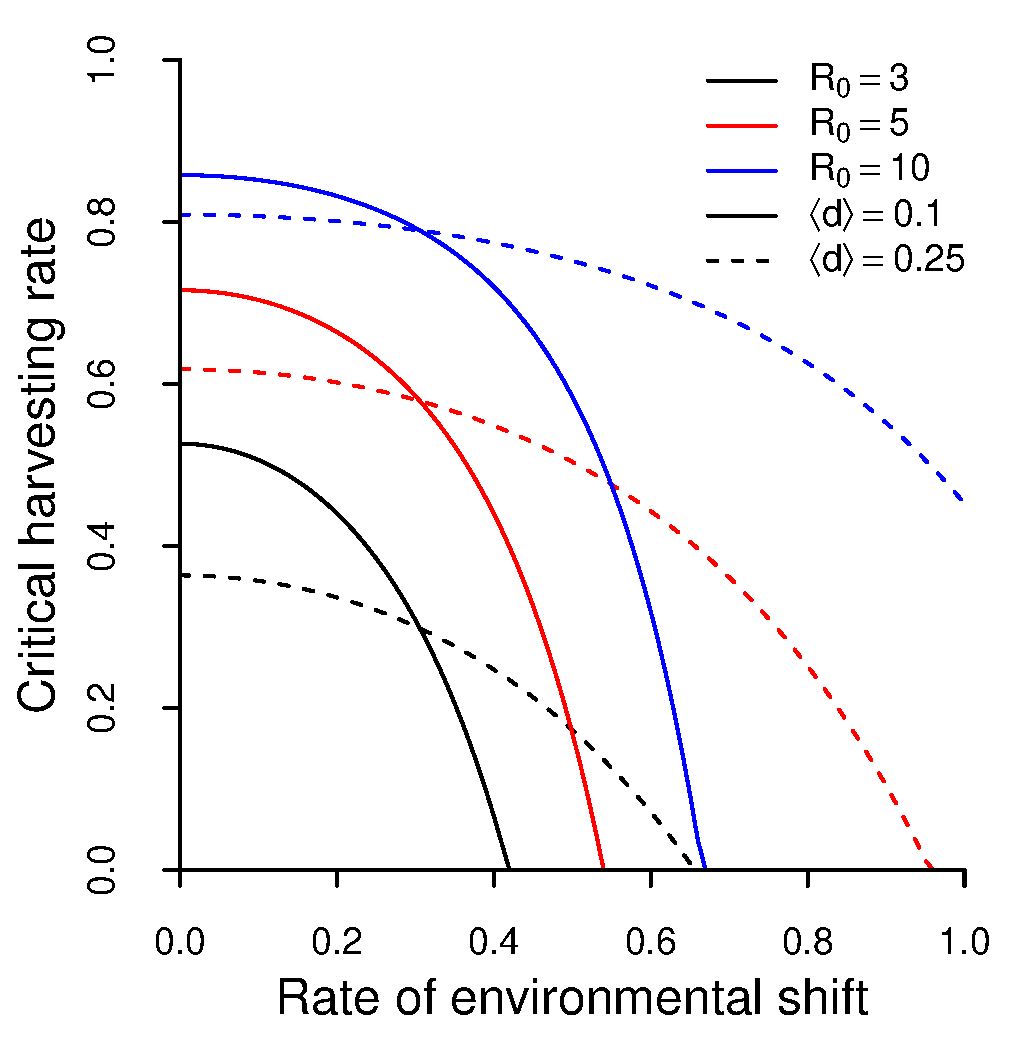
\includegraphics[width=\textwidth]{plots/critical_rates.pdf}
\end{subfigure}
\begin{subfigure}{3in}
\subcaption{\label{biomass}}
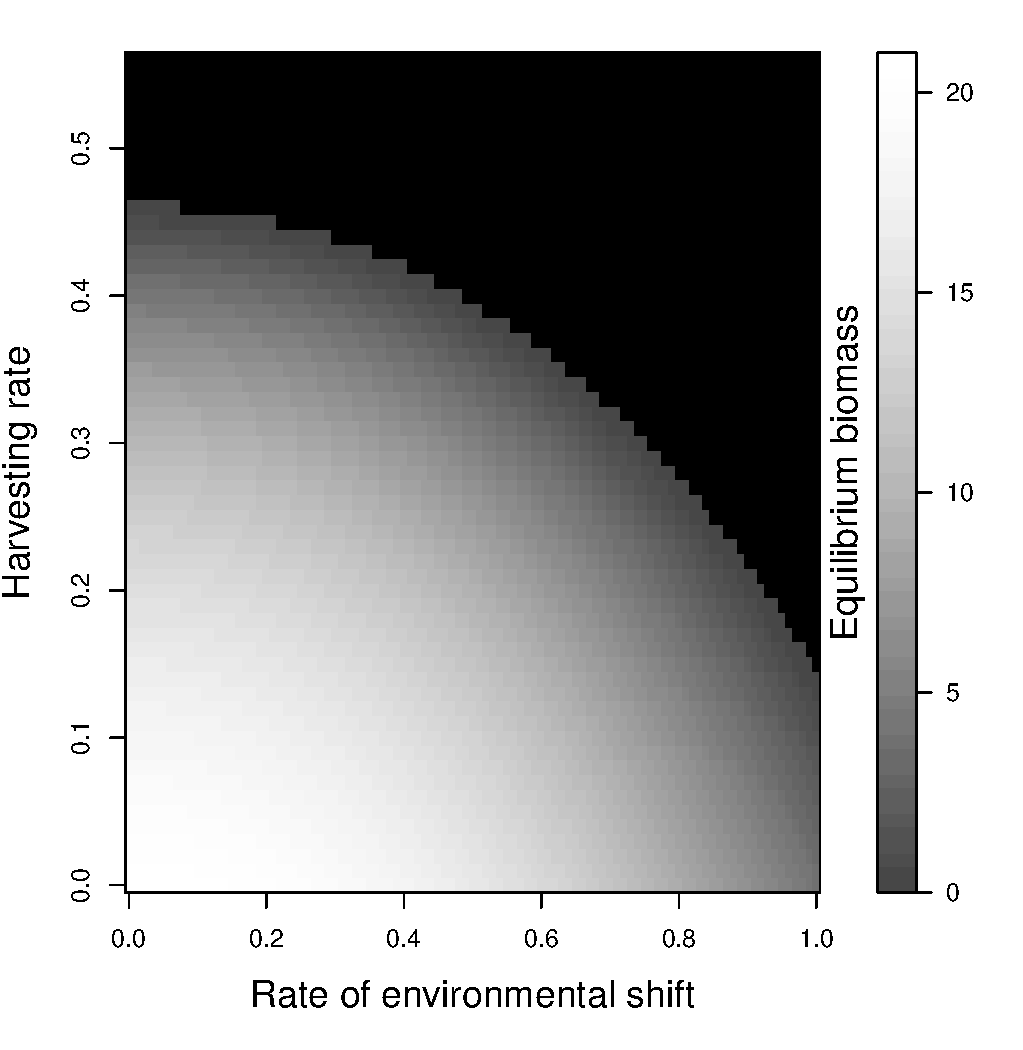
\includegraphics[width=\textwidth]{plots/eqbiomass.pdf}
\end{subfigure}

\caption{%(a) The critical harvesting rate on the y-axis as a function of the rate of environmental shift on the x-axis.  Black lines correspond to a growth rate of $R_0=3$, red to $R_0=7$, and blue to $R_0=10$.  Solid lines correspond to an average dispersal distance $\langle d \rangle =0.1$ and dashed lines correspond to an average dispersal distance $\langle d \rangle =0.25$.  (b) The equilibrium biomass of the population as a function of the rate of environmental shift on the x-axis and the harvesting rate on the y-axis. These results are from a Gaussian dispersal kernel with parameters $L=1$, $R_0=5$, $\langle d \rangle = 0.399$.    These results are from an approximated Gaussian dispersal kernel with $L=1$.
}

\label{baseline}
\end{figure}

\pagebreak

\begin{figure}[htbp]
\begin{center}
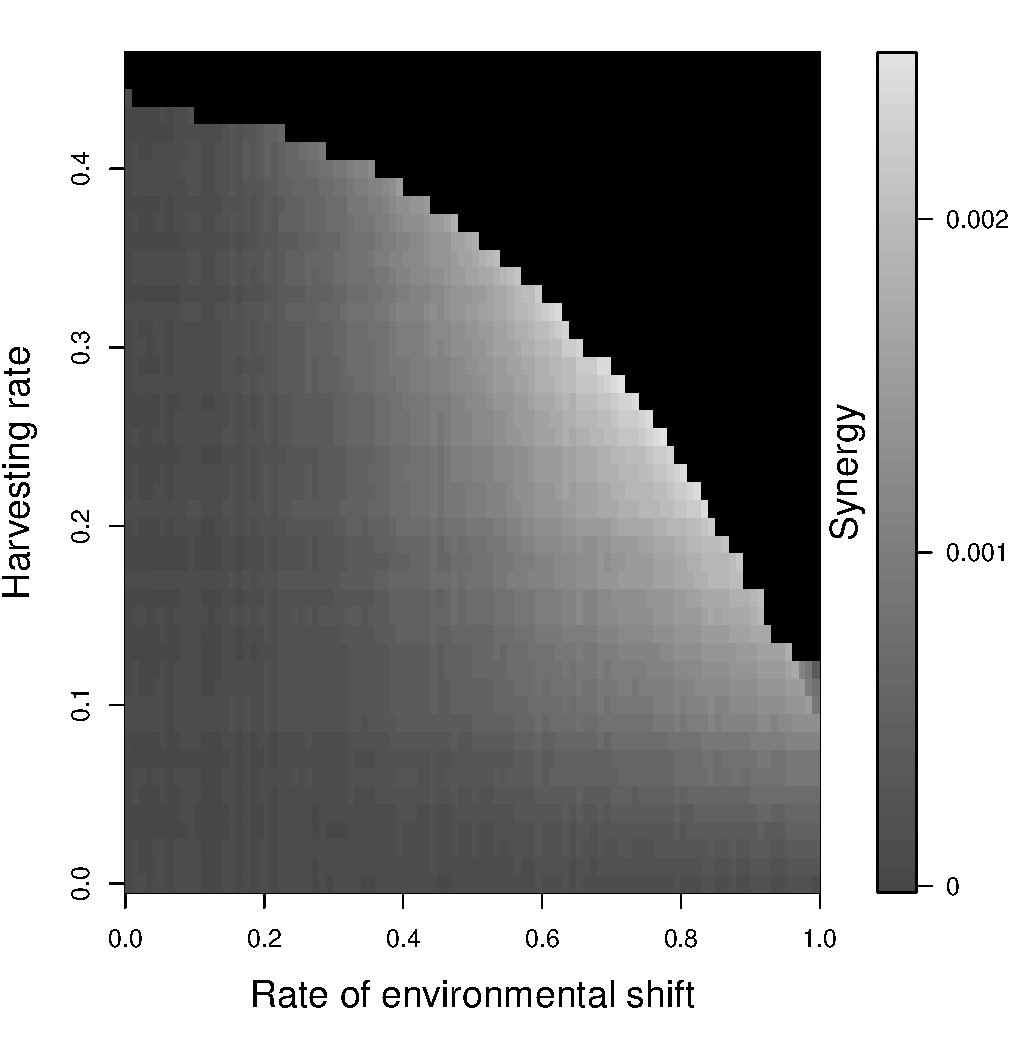
\includegraphics[width=3in]{plots/synergy.pdf}
\caption{
%Positive synergy between the two stressors.  The x-axis shows the rate of environmental shift, the y-axis shows the harvesting rate, and the color indicates the loss in biomass in the doubly stressed population in excess of the sum of the losses caused by each stressor individually, $E_\text{hc}-E_\text{h}-E_\text{c}$.  These results are from an approximated Gaussian dispersal kernel with parameters $L=1$, $R_0=5$, $\langle d \rangle = 0.399$.
}
\label{Synergy}
\end{center}
\end{figure}

\pagebreak



\pagebreak

\begin{figure}[htbp]

\begin{subfigure}{.33\textwidth}
\subcaption{}
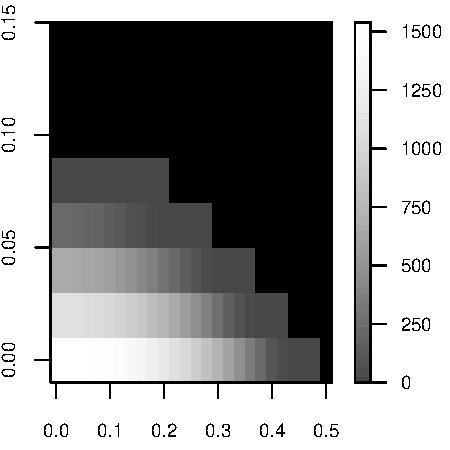
\includegraphics[width=\textwidth]{plots/eqbiomass_sim.pdf}
\label{nomang}
\end{subfigure}
\begin{subfigure}{.33\textwidth}
\subcaption{}
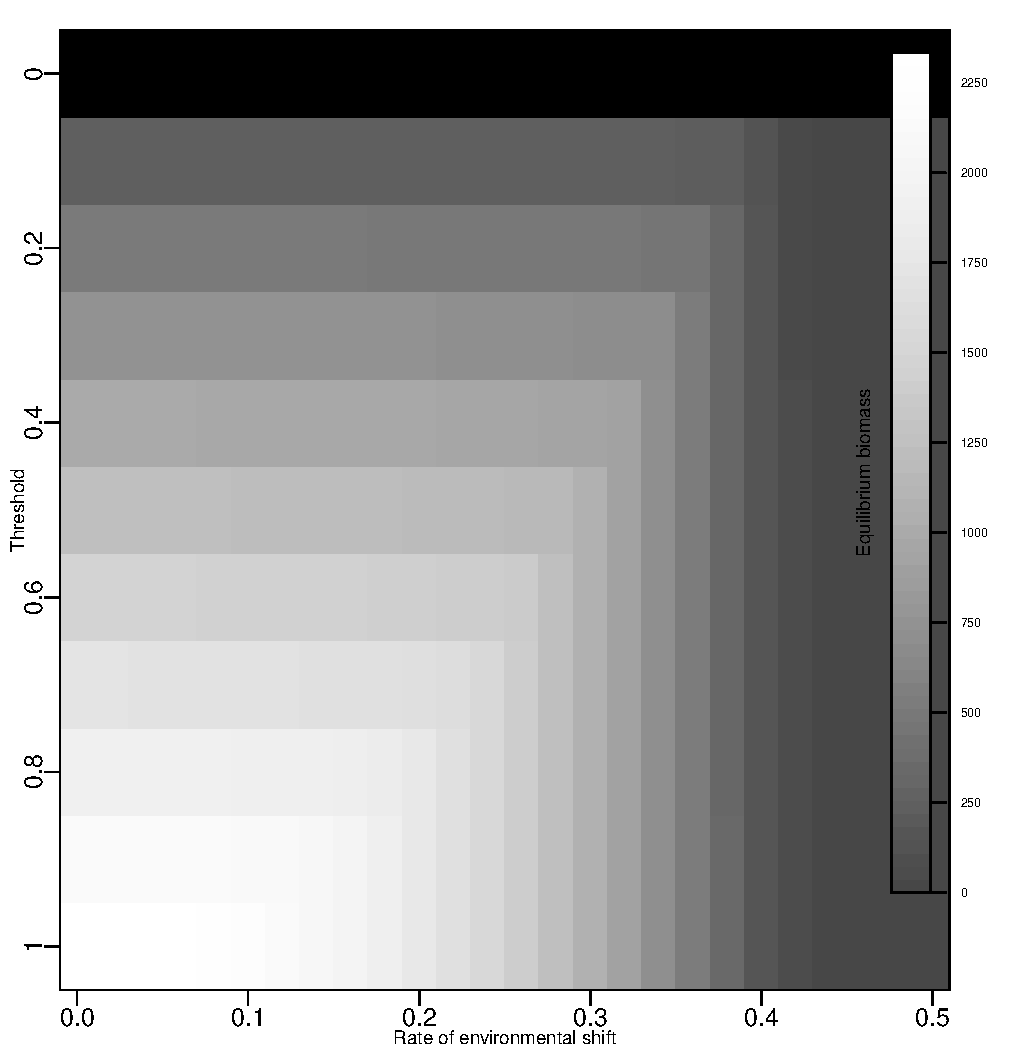
\includegraphics[width=\textwidth]{plots/eqbiomass_thresh.pdf}
\end{subfigure}
\begin{subfigure}{.33\textwidth}
\subcaption{}
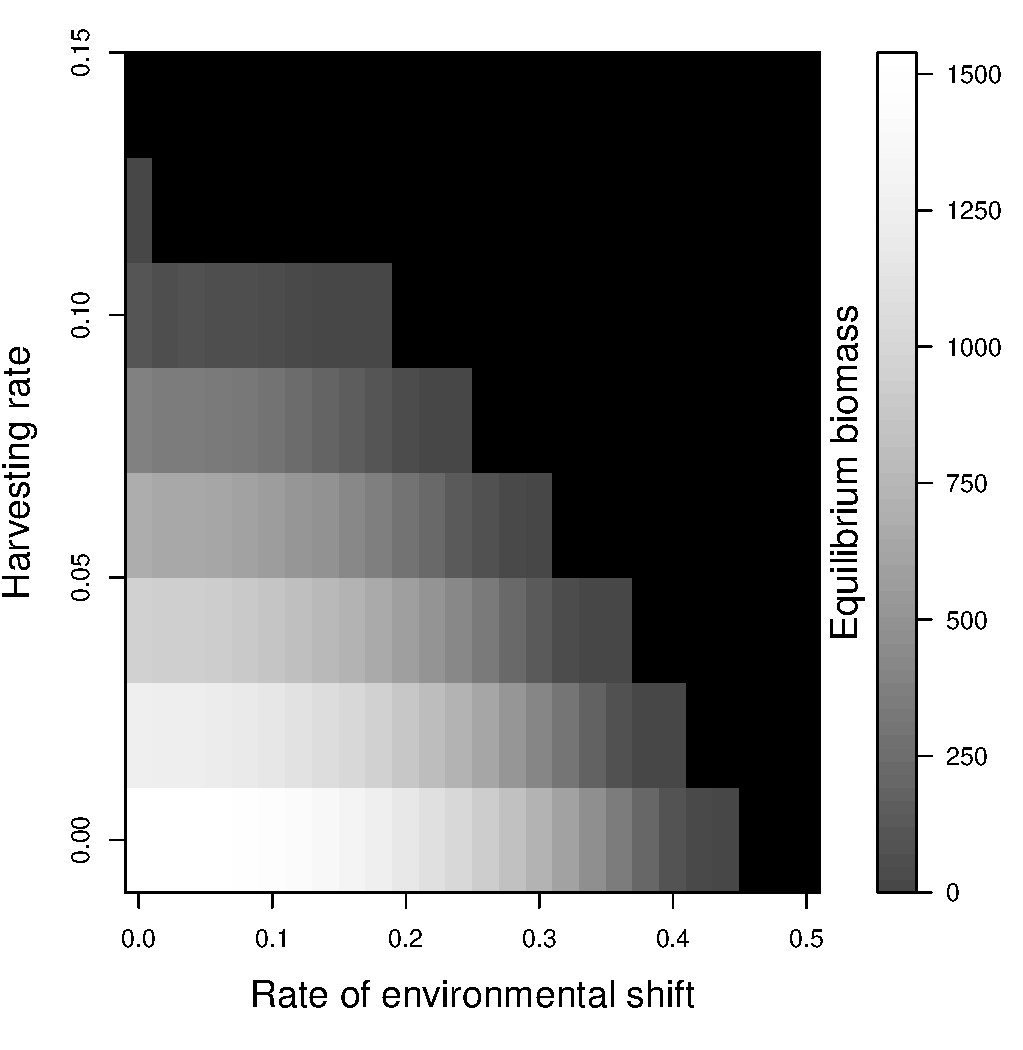
\includegraphics[width=\textwidth]{plots/eqbiomass_mpa.pdf}
\end{subfigure}
\caption{
%The equilibrium biomass of the population as a function of the rate of environmental shift on the x-axis and the harvesting rate on the y-axis with and without management strategies.  (a) No management.  (b) Threshold harvesting levels.  (c) MPAs.  These results are from a simulation with a Laplacian dispersal kernel with parameters $L=1$, $R_0=5$, $K=100$, and $\langle d \rangle =2$.
}
\label{management}
\end{figure}


\pagebreak

\section{Tables}
\begin{table}[h]
\caption{Table of variables used in the text}
\begin{tabular}{@{}lllllll@{}}
  Variable & Definition
\\\cmidrule{1-1} \cmidrule{2-2}   
$n_t(x)$ & density of fish at position $x$ at time $t$
\\ $n^*(\overline{x})$ & density of fish at equilibrium at position $\overline{x}$ relative to the patch 
\\ $k(x-y)$ & dispersal kernel, the probability of larva traveling from position $y$ to position $x$
\\ $\langle d \rangle $ & expected distance traveled by larva
\\ $f(n)$ & recruitment function, the number of offspring produced by a population of size $n$
\\ $R_0$ & intrinsic growth rate, $R_0=f'(0)$
\\ $h$ & proportion of adults harvested
\\ $L$ & patch length
\\ $c$ & rate of environmental shift
\end{tabular}
\label{variables}
\end{table}

\pagebreak



\end{spacing}
\end{document}
